\documentclass[]{article}
\usepackage[T1]{fontenc}
\usepackage{lmodern}
\usepackage{amssymb,amsmath}
\usepackage{ifxetex,ifluatex}
\usepackage{fixltx2e} % provides \textsubscript
% use upquote if available, for straight quotes in verbatim environments
\IfFileExists{upquote.sty}{\usepackage{upquote}}{}
\ifnum 0\ifxetex 1\fi\ifluatex 1\fi=0 % if pdftex
  \usepackage[utf8]{inputenc}
\else % if luatex or xelatex
  \ifxetex
    \usepackage{mathspec}
    \usepackage{xltxtra,xunicode}
  \else
    \usepackage{fontspec}
  \fi
  \defaultfontfeatures{Mapping=tex-text,Scale=MatchLowercase}
  \newcommand{\euro}{€}
\fi
% use microtype if available
\IfFileExists{microtype.sty}{\usepackage{microtype}}{}
\usepackage[margin=1in]{geometry}
\usepackage{color}
\usepackage{fancyvrb}
\newcommand{\VerbBar}{|}
\newcommand{\VERB}{\Verb[commandchars=\\\{\}]}
\DefineVerbatimEnvironment{Highlighting}{Verbatim}{commandchars=\\\{\}}
% Add ',fontsize=\small' for more characters per line
\usepackage{framed}
\definecolor{shadecolor}{RGB}{248,248,248}
\newenvironment{Shaded}{\begin{snugshade}}{\end{snugshade}}
\newcommand{\KeywordTok}[1]{\textcolor[rgb]{0.13,0.29,0.53}{\textbf{{#1}}}}
\newcommand{\DataTypeTok}[1]{\textcolor[rgb]{0.13,0.29,0.53}{{#1}}}
\newcommand{\DecValTok}[1]{\textcolor[rgb]{0.00,0.00,0.81}{{#1}}}
\newcommand{\BaseNTok}[1]{\textcolor[rgb]{0.00,0.00,0.81}{{#1}}}
\newcommand{\FloatTok}[1]{\textcolor[rgb]{0.00,0.00,0.81}{{#1}}}
\newcommand{\CharTok}[1]{\textcolor[rgb]{0.31,0.60,0.02}{{#1}}}
\newcommand{\StringTok}[1]{\textcolor[rgb]{0.31,0.60,0.02}{{#1}}}
\newcommand{\CommentTok}[1]{\textcolor[rgb]{0.56,0.35,0.01}{\textit{{#1}}}}
\newcommand{\OtherTok}[1]{\textcolor[rgb]{0.56,0.35,0.01}{{#1}}}
\newcommand{\AlertTok}[1]{\textcolor[rgb]{0.94,0.16,0.16}{{#1}}}
\newcommand{\FunctionTok}[1]{\textcolor[rgb]{0.00,0.00,0.00}{{#1}}}
\newcommand{\RegionMarkerTok}[1]{{#1}}
\newcommand{\ErrorTok}[1]{\textbf{{#1}}}
\newcommand{\NormalTok}[1]{{#1}}
\usepackage{graphicx}
% Redefine \includegraphics so that, unless explicit options are
% given, the image width will not exceed the width of the page.
% Images get their normal width if they fit onto the page, but
% are scaled down if they would overflow the margins.
\makeatletter
\def\ScaleIfNeeded{%
  \ifdim\Gin@nat@width>\linewidth
    \linewidth
  \else
    \Gin@nat@width
  \fi
}
\makeatother
\let\Oldincludegraphics\includegraphics
{%
 \catcode`\@=11\relax%
 \gdef\includegraphics{\@ifnextchar[{\Oldincludegraphics}{\Oldincludegraphics[width=\ScaleIfNeeded]}}%
}%
\ifxetex
  \usepackage[setpagesize=false, % page size defined by xetex
              unicode=false, % unicode breaks when used with xetex
              xetex]{hyperref}
\else
  \usepackage[unicode=true]{hyperref}
\fi
\hypersetup{breaklinks=true,
            bookmarks=true,
            pdfauthor={Jacques Botes},
            pdftitle={Statistical Inference: Basic inferential data analysis},
            colorlinks=true,
            citecolor=blue,
            urlcolor=blue,
            linkcolor=magenta,
            pdfborder={0 0 0}}
\urlstyle{same}  % don't use monospace font for urls
\setlength{\parindent}{0pt}
\setlength{\parskip}{6pt plus 2pt minus 1pt}
\setlength{\emergencystretch}{3em}  % prevent overfull lines
\setcounter{secnumdepth}{0}

\title{Statistical Inference: Basic inferential data analysis}
\author{Jacques Botes}
\date{September 2014}

\begin{document}

\begin{center}
\huge Statistical Inference: Basic inferential data analysis \\[0.2cm]
\end{center}
\begin{center}
\large \emph{Jacques Botes}\\[0.1cm]
\end{center}
\begin{center}
\large \emph{September 2014} \\
\end{center}
\normalsize


\begin{verbatim}
## Loading required package: ggplot2
## Loading required package: plyr
\end{verbatim}

\subsubsection{Problem Statement}\label{problem-statement}

Load the ToothGrowth data and perform some basic exploratory data
analyses Provide a basic summary of the data. Use confidence intervals
and hypothesis tests to compare tooth growth by supp and dose. (Use the
techniques from class even if there's other approaches worth
considering) State your conclusions and the assumptions needed for your
conclusions.

\subsubsection{About the data}\label{about-the-data}

The response is the length of odontoblasts (teeth) in each of 10 guinea
pigs at each of three dose levels of Vitamin C (0.5, 1, and 2 mg) with
each of two delivery methods (orange juice or ascorbic acid). A data
frame with 60 observations on 3 variables

\begin{verbatim}
##    len supp dose
## 1  4.2   VC  0.5
## 2 11.5   VC  0.5
## 3  7.3   VC  0.5
## 4  5.8   VC  0.5
## 5  6.4   VC  0.5
## 6 10.0   VC  0.5
\end{verbatim}

\begin{verbatim}
##       len       supp         dose     
##  Min.   : 4.2   OJ:30   Min.   :0.50  
##  1st Qu.:13.1   VC:30   1st Qu.:0.50  
##  Median :19.2           Median :1.00  
##  Mean   :18.8           Mean   :1.17  
##  3rd Qu.:25.3           3rd Qu.:2.00  
##  Max.   :33.9           Max.   :2.00
\end{verbatim}

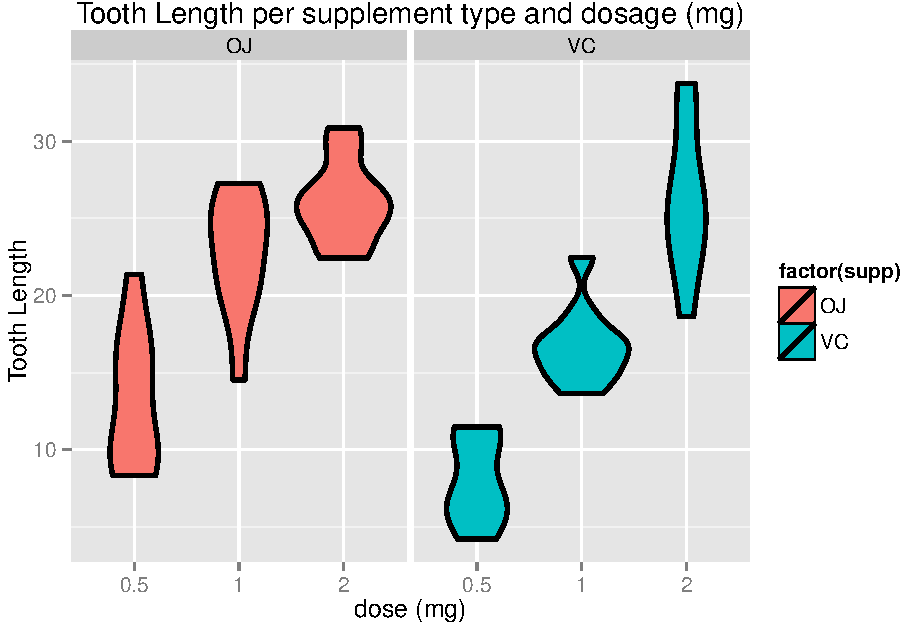
\includegraphics{./Q2_files/figure-latex/exploratory1.pdf}
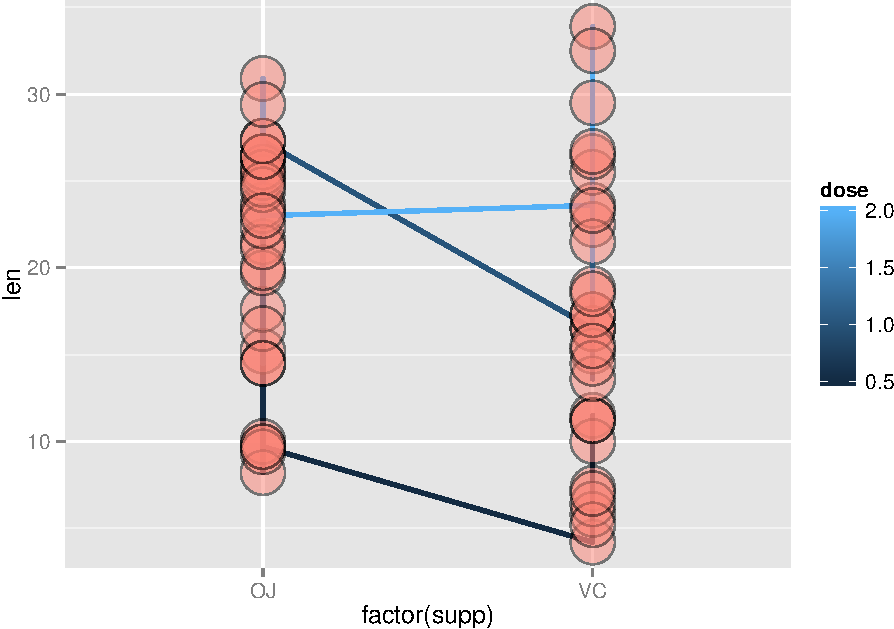
\includegraphics{./Q2_files/figure-latex/exploratory2.pdf}

\subsubsection{Summary of dataset:}\label{summary-of-dataset}

Interpreting the first graph we can see that the Orange Juice (OJ)
supplement at lower doses results in a longer tooth length. With the 2mg
dose the difference in tooth lengh is closely matched and seems to be
working equally well.

\subsubsection{Testing}\label{testing}

\paragraph{Assumptions}\label{assumptions}

\begin{itemize}
\itemsep1pt\parskip0pt\parsep0pt
\item
  The variances are different for the populations
\end{itemize}

\paragraph{Analysis}\label{analysis}

Use confidence intervals and hypothesis tests to compare tooth growth by
supp and dose.

\begin{Shaded}
\begin{Highlighting}[]
\KeywordTok{t.test}\NormalTok{(len ~}\StringTok{ }\NormalTok{supp, }\DataTypeTok{paired =} \NormalTok{F,}\DataTypeTok{var.equal=}\NormalTok{F, }\DataTypeTok{data =} \NormalTok{ToothGrowth)}
\end{Highlighting}
\end{Shaded}

\begin{verbatim}
## 
##  Welch Two Sample t-test
## 
## data:  len by supp
## t = 1.915, df = 55.31, p-value = 0.06063
## alternative hypothesis: true difference in means is not equal to 0
## 95 percent confidence interval:
##  -0.171  7.571
## sample estimates:
## mean in group OJ mean in group VC 
##            20.66            16.96
\end{verbatim}

We cannot reject the null hypothesis as there are a significant
difference in tooth length betwen OJ and VC supplement types.

Lets look at it for specific dosages

\begin{Shaded}
\begin{Highlighting}[]
\NormalTok{tooth.D05 <-}\StringTok{ }\KeywordTok{subset}\NormalTok{(ToothGrowth, dose ==}\StringTok{ }\FloatTok{0.5}\NormalTok{)}
\NormalTok{tooth.D1 <-}\StringTok{ }\KeywordTok{subset}\NormalTok{(ToothGrowth, dose ==}\StringTok{ }\FloatTok{1.0}\NormalTok{)}
\NormalTok{tooth.D2 <-}\StringTok{ }\KeywordTok{subset}\NormalTok{(ToothGrowth, dose ==}\StringTok{ }\FloatTok{2.0}\NormalTok{)}

\KeywordTok{rbind}\NormalTok{(        }
\KeywordTok{c}\NormalTok{(}\StringTok{'0.5mg conf interval'}\NormalTok{,}\KeywordTok{t.test}\NormalTok{(len ~}\StringTok{ }\NormalTok{supp, }\DataTypeTok{paired =} \NormalTok{F, }\DataTypeTok{var.equal=} \NormalTok{F,}\DataTypeTok{data =} \NormalTok{tooth.D05)$conf),}
\KeywordTok{c}\NormalTok{(}\StringTok{'1.0mg conf interval'}\NormalTok{,}\KeywordTok{t.test}\NormalTok{(len ~}\StringTok{ }\NormalTok{supp, }\DataTypeTok{paired =} \NormalTok{F, }\DataTypeTok{var.equal=} \NormalTok{F,}\DataTypeTok{data =} \NormalTok{tooth.D1)$conf),}
\KeywordTok{c}\NormalTok{(}\StringTok{'2.0mg conf interval'}\NormalTok{,}\KeywordTok{t.test}\NormalTok{(len ~}\StringTok{ }\NormalTok{supp, }\DataTypeTok{paired =} \NormalTok{F, }\DataTypeTok{var.equal=} \NormalTok{F,}\DataTypeTok{data =} \NormalTok{tooth.D2)$conf)}
\NormalTok{)}
\end{Highlighting}
\end{Shaded}

\begin{verbatim}
##      [,1]                  [,2]                [,3]              
## [1,] "0.5mg conf interval" "1.71905727146767"  "8.78094272853233"
## [2,] "1.0mg conf interval" "2.80214824916537"  "9.05785175083463"
## [3,] "2.0mg conf interval" "-3.79807046333516" "3.63807046333515"
\end{verbatim}

\subsubsection{In Conclusion:}\label{in-conclusion}

If we ignore the supplement types and just look at the difference in
dosages we notice we can reject the null hypothesis for 0.5 and 1.0mg
levels and not for the 2.0mg level. for the 2.0mg there is a significant
difference in tooth length.

Full markdown file:

\end{document}
